\documentclass[a4paper]{article}

\usepackage[ngerman]{babel}
\usepackage[utf8]{inputenc}

\usepackage[scaled]{helvet}
\renewcommand{\familydefault}{\sfdefault}
\usepackage[T1]{fontenc}

\usepackage[margin=80pt]{geometry}

\usepackage{graphicx}
\usepackage{color}
\usepackage[table,xcdraw]{xcolor}

\usepackage{enumitem}
\setlist{nosep}

\usepackage [autostyle, german]{csquotes}
\MakeOuterQuote{"}

\usepackage[hidelinks]{hyperref}
\hypersetup{colorlinks=false}

\usepackage{listings}
\definecolor{dkgreen}{rgb}{0,0.6,0}
\definecolor{gray}{rgb}{0.5,0.5,0.5}
\definecolor{mauve}{rgb}{0.58,0,0.82}

\lstset{frame=tb,
	language=Java,
	aboveskip=3mm,
	belowskip=3mm,
	showstringspaces=false,
	columns=flexible,
	basicstyle={\small\ttfamily},
	numbers=none,
	numberstyle=\tiny\color{gray},
	keywordstyle=\color{blue},
	commentstyle=\color{dkgreen},
	stringstyle=\color{mauve},
	breaklines=true,
	breakatwhitespace=true,
	tabsize=3
}


\title{\textbf{MOBPRO - Mobile Programming\\
Zusammenfassung FS 2019}}
\date{\today}
\author{Maurin D. Thalmann}

\begin{document}
	\pagenumbering{gobble}
	\maketitle
	\newpage
	\pagenumbering{arabic}
	\tableofcontents
	\newpage
	
	\section{Android 1 - Grundlagen}
	Informationen zur Androidprogrammierung können stets dem Android Developer Guide entnommen werden unter: \textit{\href{https://developer.android.com/}{developer.android.com}}
	Apps sollen grundsätzlich gegen das aktuellste API entwickelt werden, aktuell API Level 28 Android 9 "Pie".
	Im Gradle-Build-Skript werden deshalb folgende SDK-Versionen festgehalten:
	\begin{description}
		\item[\textit{minSdkVersion}] Mindestanforderung an die SDK, Minimum-Version
		\item[\textit{targetSdkVersion}] Ziel-SDK-Version, auf welcher die App lauffähig sein soll
		\item[\textit{compileSdkVersion}] Version mit welcher die App (APK) erstellt wird, meist gleich der Target-Version	
	\end{description}
	\textbf{ART (Android Runtime)} verwaltet Applikationen bzw. deren einzelne Komponenten:
	\begin{itemize}
		\item Komponente kann andere Komponente mit Intent-Mechanismus aufrufen
		\item Komponenten müssen beim System registriert werden (teilweise mit Rechten = Privileges)
		\item System verwaltet Lebenszyklus von Komponenten: Gestartet, Pausiert, Aktiv, Gestoppt, etc.
	\end{itemize}
\subsection{Komponenten}
	Applikationen sind aus Komponenten aufgebaut, die App verwendet dabei eigene Komponenten (min. eine) oder Komponenten von anderen, existierenden Applikationen.
\begin{table}[h!]
	\begin{tabular}{ l | p{11cm} }
		\textbf{\textit{Name}}               & \textbf{\textit{Beschreibung}} \\
		\hline
		\textbf{Activity}           & UI-Komponente, entspricht typischerweise einem Bildschirm \\
		\textbf{Service}            & Komponente ohne UI, Dienst läuft typischerweise im Hintergrund \\
		\textbf{Broadcast Receiver} & Event-Handler, welche auf App-interne oder systemweite Broadcast-Nachrichten reagieren \\
		\textbf{Content Provider}   & Komponente, welche Datenaustausch zwischen versch. Applikationen ermöglicht
	\end{tabular}
\end{table}

\noindent
\textbf{Activity} entspricht einem Bildschirm, stellt UI-Widgets dar, reagiert auf Benutzer-Eingabe \& -Ereignisse. Eine App besteht meist aus mehreren Activities / Bildschirmen, die auf einem "Stack" liegen. \\
Basisklasse: \textit{android.app.Activity} \\
\textbf{Service} läuft typischerweise im Hintergrund für unbeschränkte Zeit, hat keine graphische Benutzer\-schnittstelle (UI), ein UI für ein Service wird immer von einer Activity dargestellt. \\
Basisklasse: \textit{android.app.Service} \\
\textbf{Broadcast Receiver} ist eine Komponente, welche Broadcast-Nachrichten empfängt und darauf reagiert. Viele Broadcasts stammen vom System (Neue Zeitzone, Akku fast leer,...), App kann aber auch interne Broadcasts versenden. \\
Basisklasse: \textit{android.content.BroadcastReceiver}\\
\textbf{Content Provider} ist die einzige \textit{direkte} Möglichkeit zum Datenaustausch zwischen Android-Apps. Bieten Standard-API für Suchen, Löschen, Aktualisieren und Einfügen von Daten. \\
Basisklasse: \textit{android.content.ContentProvider}
\newpage
\subsection{Das Android-Manifest}
\textbf{AndroidManifest.xml} dient dazu, alle Komponenten einer Applikation dem System bekannt zu geben. Es enthält Informationen über Komponenten der Applikation, statische Rechte (Privileges), Liste mit Erlaubnissen (Permissions), ggf. Einschränkungen für Aufrufe (Intent-Filter). Es beschreibt die statischen Eigenschaften einer Applikation, beispielsweise: \\
\textit{(Diese Infos werden bei der App-Installation im System registriert, zusätzliche Infos (Version, ID, etc.) befinden sich im Gradle-Build-Skript (können build-abhängig sein))}

\begin{itemize}
	\item Java-Package-Name
	\item Benötigte Rechte (Internet, Kontakte, usw.)
	\item Deklaration der Komponenten
	\begin{itemize}
		\item Activities, Services, Broadcast Receivers, Content Providers
		\item Name (+ Basis-Package = Java Klasse)
		\item Anforderungen für Aufruf (Intent) für A, S, BR
		\item Format der gelieferten Daten für CP
	\end{itemize}
\end{itemize}
\begin{figure}[htb!]
	\centering
	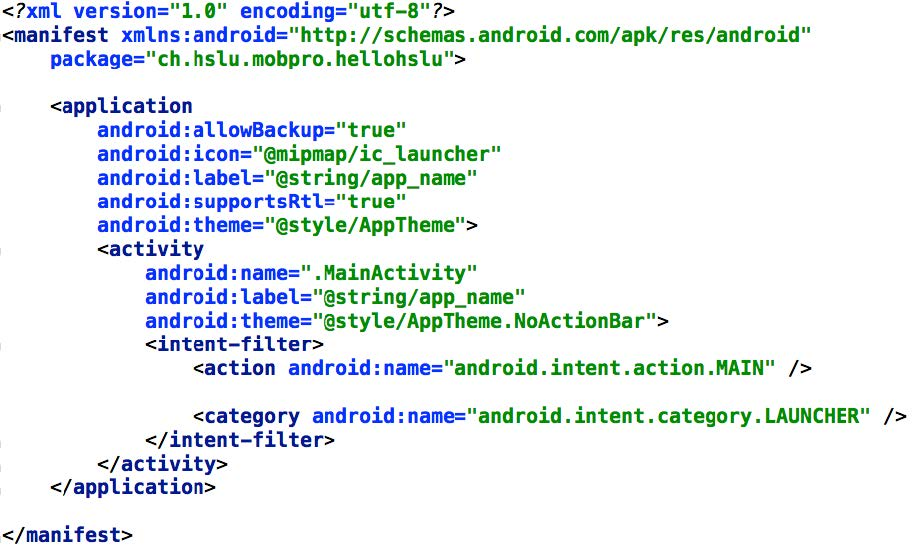
\includegraphics[width=12cm]{img/manifestxml.jpg}
	\caption{Beispiel eines Android-Manifests}
	\label{fig:manifestxml}
\end{figure}
\subsection{Activities \& Aufruf mit Intents}
Zwischen Komponenten herrscht das Prinzip der losen Kopplung:
\begin{itemize}
	\item Komponenten rufen andere Komponenten über Intents (= Nachrichten) auf
	\item Offene Kommunikation: Sender weiss nicht ob Empfänger existiert
	\item Parameterübergabe als Strings (untypisiert)
	\item Parameter: von Empfänger geprüft, geparst \& interpretiert (oder ignoriert)
	\item Keine expliziten Abhängigkeiten $\rightarrow$ Robuste Systemarchitektur
\end{itemize}
\newpage
\begin{figure}[htb!]
	\centering
	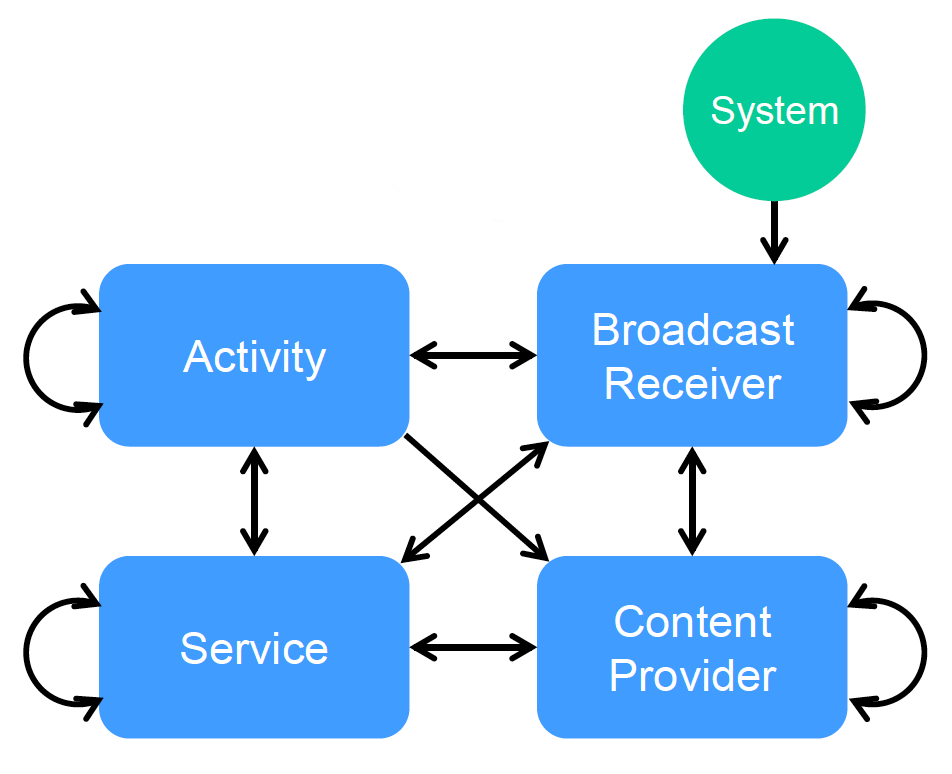
\includegraphics[width=7.5cm]{img/intents_comm.png}
	\caption{Kommunikation zwischen Komponenten mit Intents}
	\label{fig:intents_comm}	
\end{figure}
\noindent
Intents werden benutzt, um Komponenten zu benachrichtigen oder um Kontrolle zu übergeben. Es gibt folgende zwei Arten von Intents:
\begin{description}
	\item[Explizite Intents] adressieren eine Komponente direkt
	\item[Implizite Intents] beschreiben einen geeigneten Empfänger
\end{description}
\textbf{WICHTIG:} Activities müssen immer im Manifest deklariert werden, da sie sonst nicht als "public" gelten und eine Exception schmeissen. Das geht auch ganz einfach folgendermassen im Manifest unter "application":
\begin{lstlisting}
<activity android:name=".Sender" />
<activity android:name=".Receiver" />
\end{lstlisting}
\subsubsection{Beispielaufruf Expliziter Intent}
\textbf{Sender Activity:}
\begin{lstlisting}
public void onClickSendBtn(final View btn) {
	Intent intent = new Intent(this, Receiver.class); 
	// Receiver.class ist hier der explizite Empfaenger
	intent.putExtra("msg", "Hello World!");
	startActivity(intent);
}
\end{lstlisting}
\textbf{Receiver Activity:}
\begin{lstlisting}
public void onCreate(Bundle savedInstanceState) {
	// ...
	Intent intent = getIntent();
	String msg = intent.getExtras().getString("msg");
	displayMessage(msg);
}
\end{lstlisting}
\newpage
\subsubsection{Beispielaufruf Impliziter Intent}
\textbf{Sender Activity:}
\begin{lstlisting}
Intent browserCall = new Intent();
browserCall.setAction(Intent.ACTION_VIEW);
browserCall.setData(Uri.parse("http://www.hslu.ch"));
startActivity(browserCall);	
\end{lstlisting}
\textit{ACTION\_VIEW} ist hierbei kein expliziter Empfängertyp, sondern nur eine gewünschte Aktion. Die mitgege\-bene URL wird auch ein \textit{Call Parameter} genannt. Gesucht ist in diesem Fall eine Komponente, welche eine URL anzeigen/verwenden kann.\\
\subsection{Activities \& Subactivities}
\textbf{Activity Back Stack:} Activities liegen aufeinander wie ein Stapel Karten, neuste Activity zuoberst und in der Regel ist nur diese sichtbar (Durch Transparenz sind hier Ausnahmen möglich).
Durch "back" oder "finish" wird die oberste Karte entfernt und man kehrt zur zweitletzten Activity zurück. Mehrere Instanzen derselben Activity wären mehrere solche Karten, das Verhalten kann jedoch konfiguriert werden (z.Bsp. maximal eine Instant, mehrere Activities öffnen, etc.)\\
\textbf{(Sub-)Activities und Rückgabewerte:} Eine Activity kann Rückgabewerte einer anderen (Sub-)Activity erhalten.
\begin{lstlisting}
// 1. Aufruf der SubActivity mit
startActivityForResult(intent, requestId)

// 2. SubActivity setzt am Ende Resultat mit
setResult(resultCode, intent) // intent als Wrapper fuer Rueckgabewerte

// 3. SubActiity beendet sich mit
finish()

// 4. Nach Beendung der SubActivity wird folgendes im Aufrufer aufgerufen:
onActivityResult(requestId, resultCode, intent)
// resultCode: RESULT_OK, RESULT_CANCELLED
\end{lstlisting}
\subsection{Lebenszyklus \& Zustände von Applikationen/Activities}
Das System kann Applikationen bei knappem Speicher ohne Vorwarnung terminieren (nur Activities im Hintergrund, dies geschieht unbemerkt vom User, die App wird bei Zurücknavigation wiederhergestellt). Eine Applikation kann ihren Lebenszyklus demnach nicht kontrollieren und muss in der Lage sein, ihren Zustand speichern und wieder laden zu können. Applikationen durchlaufen mehrere Zustände in ihrem Lebenszyklus, Zustandsübergänge rufen Callback-Methoden auf (welche von uns überschrieben werden können.\\

\noindent
\textbf{Activity-Zustände:}
\begin{table} [h!]
	\begin{tabular}{ c | p{10cm} }
		\textbf{Zustand} & \textbf{Beschreibung} \\ \hline
		\textbf{Running} & Die Activity ist im Vordergrund auf dem Bildschirm (zuoberst auf dem Activity-Stack für die aktuelle Aufgabe). \\ \hline
		\textbf{Paused} & Die Activity hat den Fokus verloren, ist aber immer noch sichtbar für den Benutzer. \\ \hline
		\textbf{Stopped} & Die Activity ist komplett verdeckt von einer andern Activity. Der Zustand der Activity bleibt jedoch erhalten.
	\end{tabular}
\end{table}
\newpage
\subsubsection{Lifecycle einer Applikation}
\begin{figure}[h!]
	\centering
	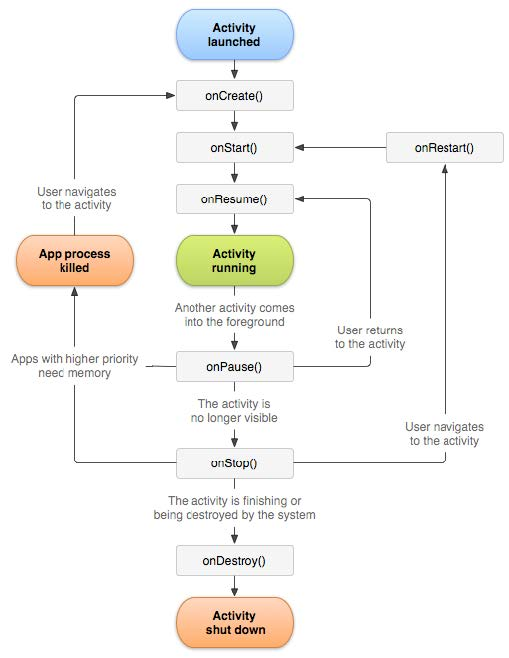
\includegraphics[width=13cm]{img/lifecycle.jpg}
	\caption{Lifecycle einer Applikation}
	\label{fig:lifecycle}
\end{figure}
\begin{figure}[h!]
	\centering
	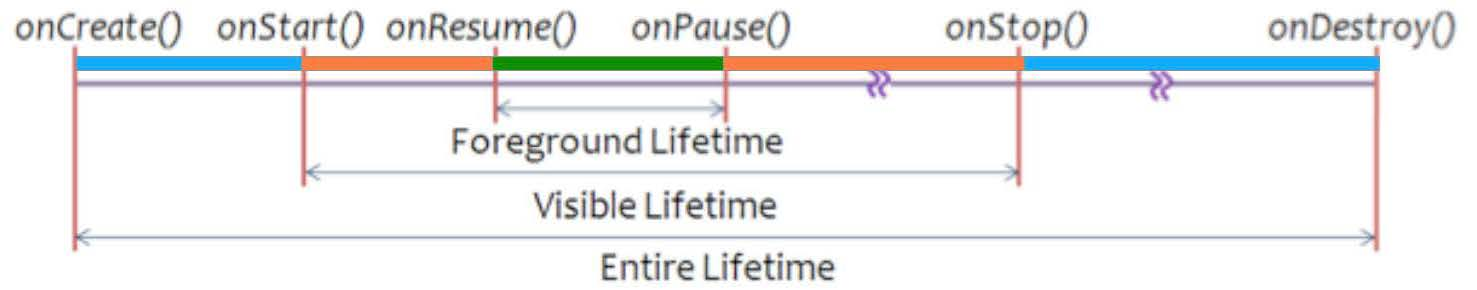
\includegraphics[width=11cm]{img/lifetime.jpg}
	\caption{Lebenszeiten der einzelnen App-Zustände}
	\label{fig:lifetime}
\end{figure}
\newpage
\subsection{Charakterisierung einer Activity}
\begin{itemize}
	\item Muss im Manifest deklariert werden
	\item GUI-Controller
	\begin{itemize}
		\item Repräsentiert eine Applikations-/Bildschirmseite
		\item Definiert Seitenlayout und GUI-Komponenten
		\item Kann aus Fragmenten ( = "Sub-Activities") aufgebaut sein
		\item Reagiert auf Benutzereingaben
		\item Beinhaltet Applikationslogik für dargestellte Seite
	\end{itemize}
\end{itemize}
\textbf{Beispiel einer Activity:}
\begin{lstlisting}
public class Demo extends Activity {
	// Called when the Activity is first created
	public void onCreate(Bundle savedInstanceState) {
		super.onCreate(savedInstanceState);
		setContentView(R.layout.main); // Definiert Layout und UI
	} 
}	
\end{lstlisting}
\subsubsection{Zustandsänderung - Hook-Methoden}
Das System benachrichtigt Activities durch Aufruf einer der folgenden Methoden der Klasse \textit{Activity}:
\begin{itemize}
	\item void onCreate(Bundle savedInstanceState)
	\item void onStart() / void onRestart()
	\item void onResume()
	\item void onPause() $\rightarrow$ \textit{bspw. Animation stoppen}
	\item void onStop()
	\item void onDestroy() $\rightarrow$ \textit{bspw. Ressourcen freigeben}
\end{itemize}
Durch das Überschreiben dieser Methoden können wir uns in den Lebenszyklus einklinken. Immer \textbf{super()} aufrufen, sonst wirft es eine Exception.
\newpage
\subsection{Android - Hinter den Kulissen}
\begin{figure}[h!]
	\centering
	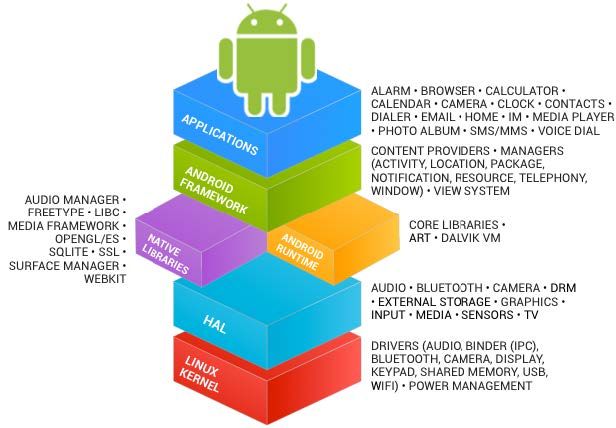
\includegraphics[width=11cm]{img/androidstack.jpg}
	\caption{Der Android-Stack}
	\label{fig:androstack}
\end{figure}
\begin{itemize}
	\item \textbf{Linux-Kernel:} OS, FS, Security, Drivers, ...
	\item \textbf{HAL (Hardware Abstraction Layer):} Camera-, Sensor-, ... Abstraktion
	\item \textbf{ART} (Android Runtime)
	\begin{itemize}
		\item Jede App in eigenem Prozess
		\item Optimiert für mehrere JVM auf low-memory Geräten
		\item Eigenes Bytecode-Format (Crosscompiling)
		\item JIT und AOT Support
	\end{itemize}
	\item \textbf{Native C/C++ Libriaries:} Zugriff via Android NDK
	\item \textbf{Android Framework:} Android Java API
	\item \textbf{Applications:} System- und eigene Apps
\end{itemize}
\newpage
\subsubsection{Android-Security-Konzept}
\textbf{Sandbox-Konzept:} 
\begin{itemize}
	\item Jede laufende Android-Anwendung hat seinen eigenen Prozess, Benutzer, ART-Instanz, Heap und Dateisystembereich $\rightarrow$ jedes App hat eigenen Linux-User
	\item Das Berechtigungssystem von Linux ist Benutzer-basiert, es betrifft deshalb sowohl den Speicherzugriff wie auch das Dateisystem. 
	\item Anwendungen signieren: erschwert Code-Manipulationen und erlaubt das Teilen einer Sandbox bei gleicher sharedUser-ID
	\item Berechtigungen werden im Manifest deklariert, kontrollierte Öffnung der Sandbox-Restriktionen
\end{itemize}
\begin{figure}[htb!]
	\centering
	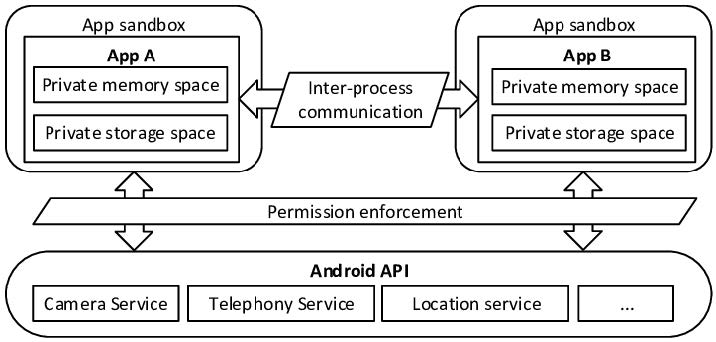
\includegraphics[width=12cm]{img/securitymodel.jpg}
	\caption{Android Security-Modell}
	\label{fig:secumodel}
\end{figure}

\newpage
\section{Android 2 - Benutzerschnittstellen}

\subsection{GUI einer Activity}

GUI wird als XML definiert, der Name resultiert in einer Konstante: \textit{\textbf{R}.layout.xxx}. Diese wird im \textit{onCreate()} einer Activity mit \textit{setContentView()} angegeben.

\begin{figure}[htb!]
	\centering
	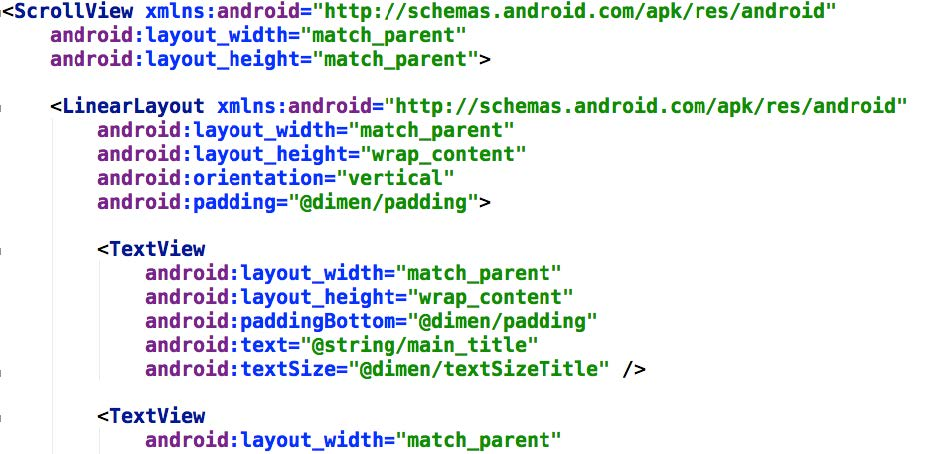
\includegraphics[width=10cm]{img/gui_xml_example.jpg}
	\caption{Beispiel eines XML für ein Layout}
	\label{fig:guixmlexamp}
\end{figure}
\noindent
Je nach Layout müssen die Elemente unterschiedlich konfiguriert werden, was bei der Arbeit mit dem Layout-Editor nicht offensichtlich, aber trotzdem gut zu wissen ist. \\
Ein Android-UI ist hierarchisch aufgebaut und besteht aus \textbf{ViewGroups} (Cointainer für Views oder weitere ViewGroups, angeordnet durch Layout) und \textbf{Views} (Widgets). Sollte auf unterschiedlichen Bildschirmgrössen gleich aussehen (Elemente deshalb \textbf{relativ} und nicht absolut positionieren)

\begin{figure}[htb!]
	\centering
	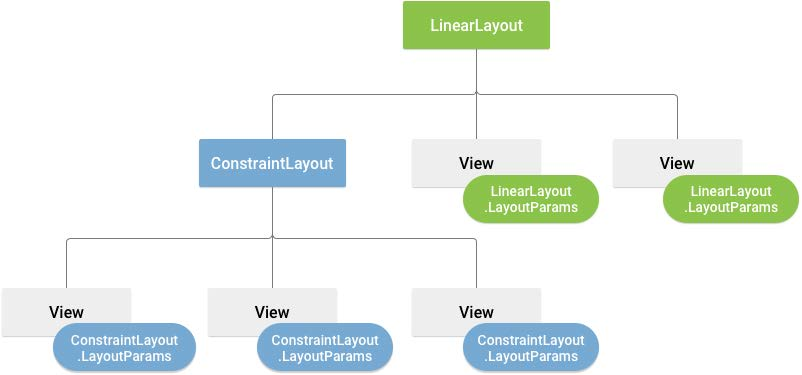
\includegraphics[width=10cm]{img/xml_layouts.jpg}
	\caption{Layout-Varianten bei Android}
	\label{fig:xmllayouts}
\end{figure}
\noindent
Schachtelung möglich, aber nicht effizient, wenn möglich immer das Constraint-Layout verwenden. Layouts spezifiziert man auf zwei verschiedene Arten:
\begin{itemize}
	\item \textbf{Statisch / Deklarativ (XML)}
	\item \textit{Grundsätzlich in MOBPRO verwendet, bietet viele Vorteile (Deklarativ, weniger umständlich als Code, Struktur eminent, Umformungen ohne Rekompilierung möglich...)}
		\begin{itemize}
			\item Deklarative Beschreibung des GUI als Komponentenbaum
			\item XML-Datei unter \textit{res/layout}
			\item Referenzen auf Bilder/Texte/etc.
			\item Typischerweise ein XML pro Activity
		\end{itemize}
	\item \textbf{Dynamisch (in Java)}
	\item \textit{Jedes XML hat eine korrespondierende Java-Klasse, XML $\rightarrow$ Java = Inflating}
		\begin{itemize}
			\item Aufbau und Definition des GUI im Java-Code
			\item Normalerweise nicht nötig: die meisten GUIs haben fixe Struktur
			\item Änderung von Eigenschaften während Laufzeit ist normal (Bsp. Visibility, Ausblenden einer View, wenn nicht benötigt)
		\end{itemize}
\end{itemize}
\newpage
\subsection{XML-Layout}
\begin{itemize}
	\item Jedes Layout ist ein eigenes XML-File
	\begin{itemize}
		\item Root-Element = View oder ViewGroup
		\item Kann Standard- oder eigene View-Klassen enthalten
	\end{itemize}
	\item XML können mit Inflater "aufgeblasen" bzw. instanziiert werden, damit eigene wiederverwendbare Komponenten/Templates/Prototypen erzeugt werden können
	\item Innere Elemente können unterhalb eines Parents via View-ID referenziert werden (\textit{findViewById()})
	\item Debugging mit dem Layout-Inspector	
\end{itemize}

\subsubsection{Constraint-Layout}
\begin{itemize}
	\item Erstellung von komplexen Layouts, ohne zu schachteln
	\item Elemente werden relativ mit Bedingungen platziert
	\begin{itemize}
		\item zu anderen Elementen
		\item zum Parent-Container
		\item Element-Chains (spread/pack)
	\end{itemize}
	\item Layout-Hilfen (Hilfslinien, Barriers)
\end{itemize}

\end{document}